\documentclass[12pt]{standalone}
\usepackage{fontspec}
\setsansfont{TeX Gyre Heros}
\newfontfamily\mfallback{DejaVu Sans}
\usepackage{tikz}
\usetikzlibrary{arrows.meta}
\newcommand{\Ufrac}[2]{\textsf{\textbf{\textit{U}}}\kern2.1pt\raisebox{-31pt}{\makebox[0pt][c]{\vbox{\offinterlineskip\hbox to 15.3pt{\hfil\fontsize{22}{24}\selectfont\textsf{\textbf{#1}}\hfil}\vskip2.1pt\hbox{\rule{15.3pt}{3.5pt}}\vskip2.1pt\hbox to 15.3pt{\hfil\fontsize{22}{24}\selectfont\textsf{\textbf{#2}}\hfil}}}}}
\newcommand{\Usub}[1]{\textsf{\textbf{\textit{U}}}\kern2.9pt\raisebox{-10.9pt}{\makebox[0pt][c]{\fontsize{22.5}{26}\selectfont\textsf{\textbf{#1}}}}}
\begin{document}
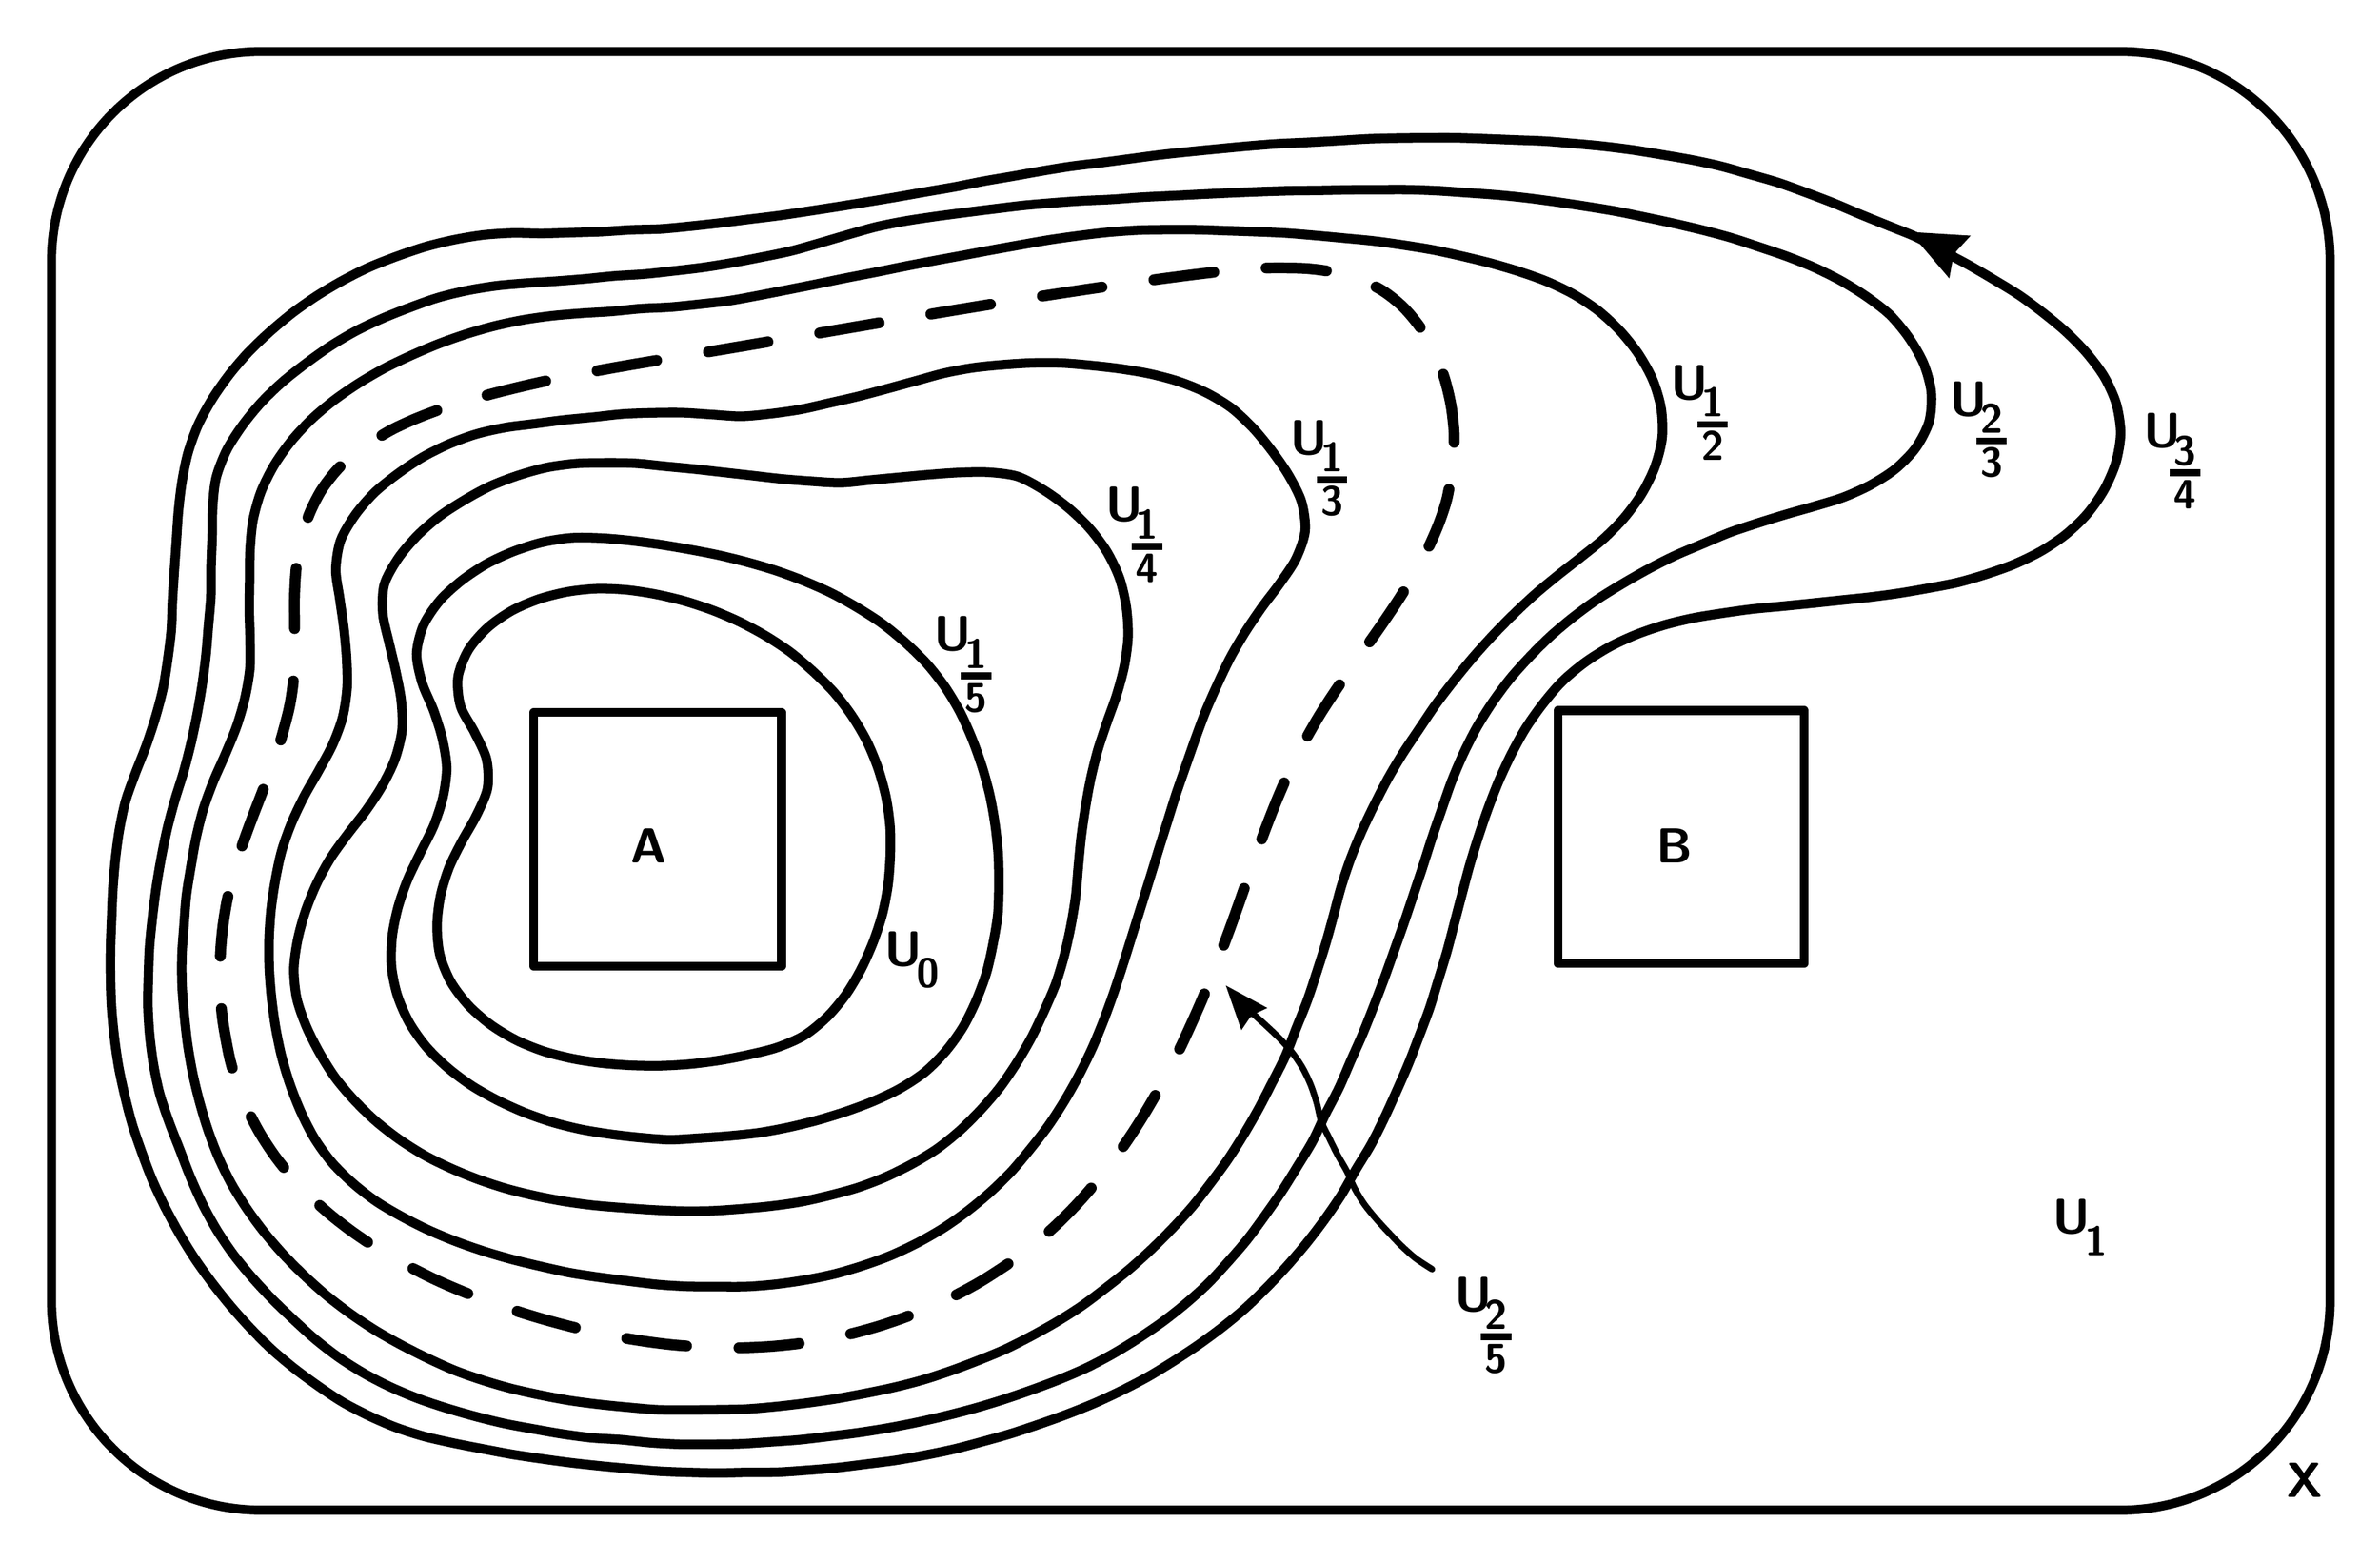
\begin{tikzpicture}[x=1pt, y=-1pt, line cap=round, line join=round]
  \path[use as bounding box] (0,0) rectangle (1182,769);

  %% ===== 外框 X（圆角矩形） =====
  \draw[line width=4.6pt, rounded corners=106pt] (16,16) rectangle (1167,753);

  %% ===== 方块 A、B =====
  \draw[line width=4.4pt] (259.7,350.0) rectangle (384.8,478.2);
  \draw[line width=4.4pt] (776.9,349.0) rectangle (901.4,476.8);

  %% ===== 实线闭合回环（由外向内） =====
  % U_{3/4} boundary (outermost solid)
  \draw[line width=4.8pt] plot[smooth cycle] coordinates {
    (957.87,109.72) (943.98,104.09) (930.08,98.46) (916.26,92.64) (902.25,87.30) (888.14,82.23) (873.74,78.05) (859.31,73.98) (844.66,70.80) (829.89,68.23) (815.09,65.82) (800.22,63.94) (785.29,62.53) (770.35,61.31) (755.37,60.72) (740.39,60.12) (725.40,59.64) (710.41,59.64) (695.42,59.79) (680.43,60.19) (665.47,61.11) (650.50,61.95) (635.52,62.64) (620.58,63.80) (605.65,65.19) (590.72,66.66) (575.82,68.26) (560.95,70.23) (546.09,72.20) (531.21,74.01) (516.40,76.38) (501.64,79.02) (486.86,81.55) (472.15,84.45) (457.37,86.99) (442.61,89.60) (427.82,92.06) (413.01,94.45) (398.19,96.73) (383.37,98.94) (368.48,100.78) (353.61,102.66) (338.70,104.29) (323.77,105.67) (308.80,106.11) (293.83,107.06) (278.85,107.53) (263.86,107.95) (248.87,107.73) (233.91,108.73) (219.13,111.18) (204.56,114.75) (190.36,119.54) (176.41,125.04) (163.02,131.75) (150.12,139.40) (137.85,148.00) (126.32,157.60) (115.49,167.96) (105.75,179.35) (97.16,191.64) (90.01,204.80) (84.94,218.90) (81.91,233.57) (80.12,248.46) (79.09,263.40) (78.05,278.35) (77.11,293.31) (76.51,308.29) (74.72,323.17) (72.33,337.97) (68.53,352.47) (63.86,366.71) (58.39,380.67) (53.41,394.81) (50.27,409.46) (48.26,424.32) (47.00,439.26) (46.36,454.24) (45.82,469.22) (45.82,484.22) (46.35,499.19) (47.76,514.11) (49.92,528.95) (53.05,543.61) (56.81,558.12) (61.65,572.31) (66.99,586.32) (73.36,599.89) (80.48,613.08) (88.36,625.84) (97.07,638.04) (106.42,649.76) (116.41,660.94) (127.00,671.55) (138.46,681.22) (150.52,690.12) (163.02,698.40) (176.32,705.32) (190.09,711.23) (204.38,715.77) (218.99,719.11) (233.71,722.01) (248.45,724.76) (263.27,727.00) (278.13,729.01) (293.03,730.64) (307.96,732.04) (322.90,733.31) (337.87,733.91) (352.86,734.21) (367.85,733.90) (382.84,733.81) (397.80,732.82) (412.74,731.55) (427.62,729.72) (442.49,727.81) (457.26,725.20) (471.94,722.14) (486.44,718.33) (500.87,714.25) (515.10,709.52) (529.21,704.46) (543.11,698.85) (556.70,692.51) (569.98,685.56) (582.78,677.75) (595.30,669.50) (607.37,660.61) (618.92,651.06) (629.72,640.66) (640.00,629.74) (649.75,618.35) (658.86,606.45) (667.33,594.08) (674.77,581.13) (682.53,568.32) (689.25,554.91) (695.46,541.27) (701.44,527.51) (706.85,513.53) (712.08,499.49) (716.52,485.16) (720.87,470.81) (724.67,456.31) (728.46,441.80) (732.32,427.31) (736.71,412.97) (741.55,398.78) (746.99,384.81) (753.31,371.21) (760.54,358.09) (769.17,345.83) (778.92,334.48) (790.38,324.82) (803.05,316.82) (816.66,310.54) (830.85,305.71) (845.42,302.21) (860.22,299.79) (875.07,297.73) (890.00,296.31) (904.91,294.81) (919.83,293.25) (934.74,291.68) (949.60,289.67) (964.37,287.13) (979.09,284.24) (993.49,280.07) (1007.59,275.01) (1021.06,268.44) (1033.48,260.06) (1044.29,249.69) (1052.86,237.44) (1058.79,223.69) (1061.21,208.97) (1059.05,194.18) (1053.00,180.49) (1044.12,168.43) (1033.65,157.72) (1022.13,148.12) (1010.06,139.23) (997.30,131.36) (984.34,123.81) (971.09,116.79)};
  % U_{2/3} boundary
  \draw[line width=4.8pt] plot[smooth cycle] coordinates {
    (659.50,552.94) (653.13,566.40) (645.40,579.25) (637.45,591.96) (628.88,604.27) (619.96,616.32) (610.18,627.69) (599.98,638.68) (588.84,648.72) (577.06,658.00) (564.67,666.43) (551.86,674.23) (538.58,681.19) (524.79,687.10) (510.75,692.36) (496.56,697.21) (482.20,701.54) (467.69,705.33) (453.07,708.66) (438.35,711.51) (423.53,713.85) (408.65,715.72) (393.76,717.46) (378.81,718.55) (363.85,719.50) (348.86,719.72) (333.86,719.72) (318.89,718.95) (303.97,717.42) (289.01,716.46) (274.14,714.51) (259.36,711.95) (244.63,709.18) (230.06,705.61) (215.65,701.47) (201.43,696.70) (187.59,690.94) (174.24,684.10) (161.55,676.13) (149.64,667.01) (138.51,656.97) (127.71,646.57) (117.51,635.58) (108.01,623.97) (99.60,611.57) (92.36,598.43) (86.20,584.76) (80.79,570.77) (75.37,556.79) (70.66,542.56) (67.54,527.90) (65.61,513.03) (64.72,498.07) (64.96,483.08) (65.55,468.10) (67.03,453.18) (68.93,438.30) (71.43,423.52) (74.45,408.83) (78.29,394.34) (82.74,380.02) (86.49,365.51) (89.58,350.83) (92.11,336.05) (94.03,321.18) (95.28,306.24) (96.52,291.30) (96.62,276.30) (97.16,261.32) (97.41,246.33) (99.16,231.45) (104.49,217.47) (112.53,204.83) (122.04,193.23) (132.83,182.84) (144.60,173.53) (156.83,164.87) (169.75,157.25) (183.30,150.82) (197.23,145.28) (211.39,140.34) (225.96,136.79) (240.75,134.39) (255.69,133.05) (270.65,132.07) (285.59,130.88) (300.51,129.41) (315.48,128.47) (330.38,126.87) (345.26,125.09) (360.07,122.72) (374.80,119.90) (389.48,116.84) (403.93,112.80) (418.31,108.58) (432.76,104.57) (447.47,101.65) (462.30,99.40) (477.17,97.43) (492.05,95.57) (506.94,93.80) (521.88,92.50) (536.82,91.44) (551.80,90.74) (566.76,89.64) (581.74,88.91) (596.72,88.15) (611.70,87.45) (626.68,86.83) (641.67,86.37) (656.66,86.19) (671.65,85.91) (686.65,85.83) (701.65,85.83) (716.63,86.39) (731.59,87.43) (746.54,88.51) (761.45,90.05) (776.31,92.03) (791.14,94.26) (805.94,96.69) (820.64,99.67) (835.31,102.81) (849.91,106.24) (864.39,110.12) (878.65,114.78) (892.84,119.63) (906.74,125.27) (920.15,131.97) (932.88,139.88) (944.69,149.10) (954.25,160.62) (961.66,173.63) (965.53,188.06) (964.46,202.94) (957.74,216.25) (947.33,227.01) (934.74,235.10) (921.07,241.27) (906.75,245.71) (892.33,249.82) (878.00,254.25) (863.78,259.01) (849.95,264.82) (836.15,270.68) (822.76,277.43) (809.72,284.83) (796.98,292.74) (784.88,301.60) (773.39,311.23) (762.72,321.77) (752.72,332.94) (743.80,344.98) (735.84,357.70) (729.06,371.06) (723.20,384.87) (718.24,399.01) (713.37,413.19) (708.81,427.48) (704.08,441.71) (699.32,455.93) (694.32,470.07) (689.28,484.20) (683.97,498.22) (678.42,512.15) (672.34,525.86) (666.39,539.63)};
  % U_{1/2} boundary
  \draw[line width=4.8pt] plot[smooth cycle] coordinates {
    (564.76,106.29) (579.72,106.01) (594.69,106.05) (609.65,106.56) (624.61,107.08) (639.55,107.76) (654.47,108.97) (669.37,110.35) (684.27,111.80) (699.10,113.85) (713.87,116.26) (728.50,119.43) (743.05,122.98) (757.41,127.20) (771.49,132.25) (784.96,138.76) (797.41,147.04) (808.38,157.22) (817.69,168.92) (824.90,182.02) (829.08,196.34) (829.59,211.23) (826.00,225.73) (819.46,239.17) (810.69,251.30) (800.26,261.99) (788.66,271.45) (776.88,280.69) (765.37,290.25) (754.42,300.46) (743.93,311.14) (733.92,322.27) (724.43,333.84) (715.36,345.76) (706.97,358.15) (698.65,370.60) (691.01,383.47) (684.14,396.77) (677.73,410.29) (672.09,424.16) (667.38,438.36) (663.52,452.83) (659.51,467.25) (655.01,481.52) (650.27,495.72) (644.74,509.63) (639.31,523.53) (632.62,536.92) (625.75,550.21) (618.26,563.18) (610.23,575.81) (601.39,587.89) (592.19,599.69) (582.10,610.74) (571.50,621.32) (560.38,631.33) (548.66,640.65) (536.69,649.63) (524.07,657.69) (511.02,665.01) (497.65,671.76) (483.82,677.48) (469.81,682.74) (455.57,687.36) (441.07,691.07) (426.41,694.11) (411.69,696.82) (396.87,698.93) (382.00,700.66) (367.09,701.92) (352.13,702.26) (337.16,702.38) (322.19,702.26) (307.29,701.02) (292.40,699.53) (277.56,697.56) (262.85,694.81) (248.24,691.54) (233.87,687.37) (219.75,682.41) (206.09,676.29) (192.72,669.57) (179.69,662.19) (167.23,653.90) (155.33,644.83) (144.15,634.87) (133.57,624.29) (123.78,612.97) (114.88,600.94) (106.96,588.23) (100.37,574.80) (95.03,560.83) (90.74,546.49) (87.25,531.93) (84.73,517.19) (83.06,502.31) (81.94,487.39) (81.91,472.42) (82.95,457.50) (84.13,442.59) (86.45,427.80) (89.09,413.07) (92.78,398.56) (97.90,384.50) (103.94,370.80) (109.55,356.93) (113.75,342.56) (116.21,327.82) (116.29,312.85) (115.91,297.89) (116.09,282.93) (116.29,267.96) (117.75,253.09) (121.75,238.67) (128.34,225.26) (136.94,213.03) (147.10,202.05) (158.52,192.37) (170.82,183.85) (183.74,176.29) (197.22,169.78) (210.99,163.92) (225.09,158.91) (239.48,154.77) (254.12,151.65) (268.94,149.55) (283.85,148.27) (298.79,147.35) (313.68,145.92) (328.62,145.17) (343.51,143.67) (358.38,141.94) (373.11,139.28) (387.80,136.42) (402.48,133.50) (417.15,130.48) (431.84,127.64) (446.51,124.66) (461.22,121.84) (475.94,119.13) (490.65,116.37) (505.39,113.73) (520.14,111.17) (534.96,109.08) (549.83,107.34)};
  % U_{1/3} boundary
  \draw[line width=4.8pt] plot[smooth cycle] coordinates {
    (511.22,173.38) (526.18,173.40) (541.10,174.62) (555.96,176.32) (570.71,178.83) (585.18,182.67) (599.05,188.28) (611.85,195.99) (622.84,206.14) (632.37,217.66) (640.85,229.99) (647.41,243.43) (649.27,258.17) (644.64,272.27) (636.47,284.80) (627.48,296.76) (619.09,309.16) (611.54,322.08) (605.06,335.56) (599.04,349.27) (593.79,363.28) (588.84,377.41) (583.95,391.56) (579.48,405.84) (575.02,420.13) (570.63,434.44) (566.18,448.73) (561.73,463.02) (557.27,477.31) (552.60,491.52) (547.48,505.59) (541.76,519.42) (535.19,532.87) (527.86,545.91) (519.74,558.49) (510.60,570.34) (500.97,581.79) (490.28,592.25) (478.77,601.83) (466.54,610.45) (453.56,617.90) (440.03,624.29) (425.97,629.42) (411.61,633.64) (396.96,636.67) (382.15,638.82) (367.23,640.02) (352.26,640.07) (337.30,639.94) (322.36,639.01) (307.50,637.25) (292.65,635.34) (277.86,633.05) (263.24,629.85) (248.70,626.33) (234.33,622.15) (220.20,617.20) (206.39,611.44) (193.03,604.70) (180.15,597.08) (168.34,587.91) (157.70,577.40) (148.93,565.28) (142.07,551.99) (136.56,538.08) (132.25,523.75) (129.20,509.10) (127.16,494.28) (126.01,479.36) (125.91,464.41) (126.91,449.48) (129.08,434.66) (132.24,420.04) (137.20,405.94) (143.59,392.41) (150.98,379.39) (158.03,366.19) (163.13,352.14) (165.32,337.35) (165.06,322.39) (163.72,307.49) (161.64,292.67) (159.63,277.85) (161.99,263.17) (169.38,250.20) (179.14,238.89) (190.76,229.46) (203.20,221.15) (216.57,214.43) (230.62,209.30) (245.20,206.01) (260.05,204.09) (274.89,202.18) (289.79,200.74) (304.67,199.16) (319.62,198.58) (334.57,198.50) (349.51,199.43) (364.44,200.33) (379.34,199.02) (394.15,196.90) (408.76,193.65) (423.35,190.30) (437.82,186.48) (452.26,182.53) (466.69,178.59) (481.40,175.83) (496.29,174.29)};
  % U_{1/4} boundary
  \draw[line width=4.8pt] plot[smooth cycle] coordinates {
    (280.71,224.22) (295.65,223.84) (310.60,224.07) (325.48,225.53) (340.36,226.95) (355.22,228.62) (370.09,230.29) (384.95,231.97) (399.85,233.15) (414.77,233.92) (429.66,232.53) (444.55,231.13) (459.44,229.78) (474.34,228.75) (489.29,228.60) (504.04,230.72) (517.27,237.61) (529.38,246.38) (540.16,256.72) (549.09,268.69) (555.52,282.16) (558.92,296.70) (559.82,311.61) (557.94,326.42) (554.12,340.86) (549.15,354.97) (544.47,369.17) (540.89,383.69) (538.20,398.41) (536.10,413.21) (534.66,428.10) (533.33,442.99) (530.93,457.75) (527.70,472.35) (523.42,486.66) (517.60,500.44) (511.14,513.93) (503.65,526.87) (495.22,539.22) (485.51,550.58) (474.91,561.14) (463.26,570.50) (450.47,578.22) (437.05,584.81) (423.07,590.10) (408.64,594.05) (394.05,597.30) (379.24,599.39) (364.35,600.78) (349.43,601.77) (334.48,601.89) (319.53,601.28) (304.62,600.22) (289.72,598.96) (274.90,596.96) (260.22,594.13) (245.70,590.52) (231.49,585.86) (217.64,580.24) (204.24,573.60) (191.60,565.62) (179.81,556.44) (169.09,546.02) (159.43,534.61) (151.44,521.98) (144.73,508.62) (139.91,494.49) (138.42,479.64) (140.35,464.82) (144.29,450.40) (149.89,436.54) (157.06,423.42) (165.77,411.27) (174.93,399.44) (183.11,386.93) (189.55,373.45) (193.07,358.96) (192.68,344.05) (189.96,329.35) (186.54,314.79) (183.38,300.18) (184.09,285.38) (191.03,272.20) (200.65,260.76) (211.88,250.92) (224.40,242.76) (237.54,235.63) (251.50,230.27) (265.90,226.26)};
  % U_{1/5} boundary
  \draw[line width=4.8pt] plot[smooth cycle] coordinates {
    (278.52,261.75) (293.53,261.86) (308.50,263.15) (323.40,265.11) (338.21,267.60) (352.96,270.47) (367.55,274.06) (381.96,278.30) (396.06,283.50) (409.80,289.59) (422.93,296.88) (435.54,305.04) (447.17,314.55) (457.91,325.05) (467.20,336.84) (474.93,349.72) (481.09,363.42) (486.14,377.57) (490.06,392.07) (492.67,406.87) (494.24,421.81) (494.53,436.83) (494.04,451.85) (491.64,466.68) (488.33,481.33) (483.14,495.43) (476.48,508.89) (467.72,521.08) (457.12,531.71) (444.60,539.99) (431.03,546.44) (416.96,551.69) (402.59,556.07) (387.99,559.62) (373.21,562.33) (358.27,563.93) (343.29,565.01) (328.29,565.81) (313.32,564.75) (298.39,563.04) (283.56,560.61) (268.98,556.98) (254.80,552.04) (241.12,545.83) (228.06,538.41) (216.04,529.40) (205.33,518.88) (196.69,506.62) (190.71,492.85) (187.73,478.15) (188.10,463.15) (191.04,448.42) (195.96,434.23) (202.43,420.67) (209.08,407.20) (213.73,392.94) (215.65,378.06) (213.45,363.23) (209.00,348.88) (203.23,335.01) (200.44,320.35) (203.91,305.87) (212.19,293.37) (223.26,283.24) (235.75,274.92) (249.38,268.60) (263.69,264.05)};
  % U_0 boundary
  \draw[line width=4.8pt] plot[smooth cycle] coordinates {
    (291.63,287.42) (306.54,288.02) (321.29,290.24) (335.81,293.67) (349.99,298.35) (363.70,304.24) (376.86,311.30) (389.30,319.55) (400.68,329.21) (411.23,339.76) (420.30,351.62) (427.86,364.48) (433.56,378.27) (437.52,392.65) (439.57,407.44) (439.68,422.37) (438.54,437.23) (435.69,451.88) (431.03,466.06) (424.95,479.68) (417.30,492.49) (407.72,503.90) (396.11,513.25) (382.49,519.25) (368.02,522.92) (353.36,525.72) (338.55,527.61) (323.64,528.47) (308.73,528.25) (293.85,527.11) (279.10,524.83) (264.64,521.14) (250.80,515.56) (238.02,507.87) (226.77,498.09) (217.79,486.19) (212.19,472.41) (210.76,457.59) (212.46,442.80) (216.76,428.52) (223.31,415.11) (230.60,402.08) (236.24,388.29) (235.76,373.59) (229.70,359.98) (222.66,346.83) (221.35,332.08) (226.66,318.28) (236.40,307.02) (248.61,298.50) (262.33,292.63) (276.79,288.98)};
  % ===== 虚线回环 U_{2/5} =====
  \draw[line width=5.5pt, dash pattern=on 30.5pt off 26.5pt] plot[smooth cycle] coordinates {
    (724.23,223.33) (724.51,209.00) (722.91,194.58) (719.47,180.49) (714.22,167.21) (707.21,155.17) (698.48,144.84) (688.07,136.67) (676.07,130.92) (662.79,127.35) (648.53,125.59) (628.56,125.43) (613.29,126.47) (598.13,128.11) (583.39,129.97) (569.18,131.87) (555.31,133.80) (541.59,135.79) (527.84,137.85) (514.02,139.98) (500.14,142.17) (486.21,144.42) (467.57,147.48) (453.57,149.82) (439.56,152.18) (425.54,154.56) (411.54,156.95) (397.57,159.34) (383.63,161.72) (369.74,164.08) (355.91,166.41) (342.15,168.70) (328.47,170.97) (310.30,174.01) (296.67,176.40) (282.99,178.95) (269.21,181.74) (255.30,184.82) (241.20,188.27) (226.94,192.16) (212.78,196.65) (199.04,201.91) (186.05,208.10) (170.46,218.10) (160.48,227.12) (152.34,237.65) (146.24,249.70) (142.06,262.94) (139.64,276.96) (138.76,291.36) (138.79,305.89) (138.86,320.33) (138.13,334.46) (135.98,348.14) (131.24,365.85) (126.74,378.90) (121.79,391.90) (116.75,404.99) (111.96,418.29) (107.75,431.95) (104.47,446.08) (102.27,460.64) (101.19,475.45) (101.24,490.32) (102.45,505.04) (105.90,524.14) (109.88,537.80) (115.09,550.71) (121.46,562.82) (128.91,574.15) (137.36,584.73) (146.72,594.59) (156.92,603.75) (167.86,612.23) (179.46,620.06) (191.63,627.26) (208.62,635.92) (221.82,641.75) (235.32,647.04) (249.02,651.79) (262.86,656.06) (276.75,659.84) (290.66,663.13) (304.57,665.89) (318.50,668.09) (332.43,669.70) (350.99,670.85) (364.90,670.93) (378.80,670.30) (392.67,668.92) (406.51,666.76) (420.32,663.78) (434.04,659.98) (447.60,655.37) (460.90,649.97) (473.85,643.81) (486.36,636.89) (502.20,626.53) (513.33,617.94) (523.79,608.67) (533.62,598.80) (542.84,588.35) (551.50,577.40) (559.62,565.98) (567.25,554.15) (574.40,541.97) (581.12,529.47) (587.44,516.72) (595.30,499.41) (600.82,486.26) (606.05,473.03) (611.03,459.77) (615.79,446.52) (620.42,433.33) (625.05,420.22) (629.84,407.21) (634.92,394.33) (640.43,381.60) (646.52,369.04) (655.77,352.61) (663.55,340.51) (671.79,328.51) (680.24,316.56) (688.64,304.58) (696.74,292.49) (704.28,280.23) (711.00,267.73) (716.65,254.90) (720.97,241.68) (724.23,223.33)};
  % ===== U_{2/5} 引导线与箭头 =====
  \draw[-{Stealth[length=22pt,width=16.5pt,inset=2pt]}, line width=3.2pt] plot[smooth] coordinates {
    (713.37,631.25) (705.27,625.92) (698.19,619.69) (691.58,612.87) (685.04,605.73) (679.00,598.22) (674.14,590.18) (670.35,581.78) (665.71,573.63) (661.45,565.06) (657.42,556.66) (655.14,547.37) (652.11,538.22) (648.01,529.62) (642.73,521.79) (636.41,514.71) (629.46,508.08) (622.30,501.59) (615.38,494.94) (609.12,487.82)};
  %% ===== 外层曲线上的箭头 =====
  \draw[-{Stealth[length=28pt,width=23pt,inset=3pt]}, line width=4.8pt] (963.1,111.4) -- (954.5,107.1);

  %% ===== 标签（一个标签 = 一个节点；实测墨迹基线定位） =====
  \node[anchor=base west,inner sep=0pt,font=\fontsize{30}{34}\selectfont] at (833.7,191.7) {\Ufrac{1}{2}};
  \node[anchor=base west,inner sep=0pt,font=\fontsize{30}{34}\selectfont] at (974.7,200.0) {\Ufrac{2}{3}};
  \node[anchor=base west,inner sep=0pt,font=\fontsize{30}{34}\selectfont] at (1072.5,216.2) {\Ufrac{3}{4}};
  \node[anchor=base west,inner sep=0pt,font=\fontsize{30}{34}\selectfont] at (641.5,219.5) {\Ufrac{1}{3}};
  \node[anchor=base west,inner sep=0pt,font=\fontsize{30}{34}\selectfont] at (548.1,253.3) {\Ufrac{1}{4}};
  \node[anchor=base west,inner sep=0pt,font=\fontsize{30}{34}\selectfont] at (461.7,318.8) {\Ufrac{1}{5}};
  \node[anchor=base west,inner sep=0pt,font=\fontsize{30}{34}\selectfont] at (436.6,478.1) {\Usub{0}};
  \node[anchor=base west,inner sep=0pt,font=\fontsize{30}{34}\selectfont] at (1026.6,613.3) {\Usub{1}};
  \node[anchor=base west,inner sep=0pt,font=\fontsize{30}{34}\selectfont] at (724.5,652.5) {\Ufrac{2}{5}};
  \node[anchor=base,inner sep=0pt,font=\fontsize{30}{34}\selectfont] at (317.6,426.1) {\textsf{\textbf{\textit{A}}}};
  \node[anchor=base,inner sep=0pt,font=\fontsize{30}{34}\selectfont] at (836.0,426.1) {\textsf{\textbf{\textit{B}}}};
  \node[anchor=base,inner sep=0pt,font=\fontsize{30}{34}\selectfont] at (1154.2,746.5) {\textsf{\textbf{\textit{X}}}};
\end{tikzpicture}
\end{document}
